\section{Reciprocal Consistency}
\label{sec:recipr-cons}

In the property graph data model edges have direction, each edge having a pair of \emph{source} and \emph{destination} vertices.
In the storage layer, edge information is stored with \textbf{both} the source and destination vertices.
This, as we explain next, allows an edge to be traversed in both directions and thus facilitates improved query performance.

Consider, for example, the statement that Tolkien \textit{wrote} The Hobbit.
It is expressed using vertices \emph{a} and \emph{b}, for Tolkien and The Hobbit respectively, and an edge \textit{wrote} running from \emph{a} (source) to \emph{b} (destination). The logical representation of the edge is given in Figure \ref{rc-edge}.

Using openCypher \cite{openCypher} this can be represented by:
\begin{Verbatim}[commandchars=\\\{\},fontsize=\small,xleftmargin=.2in]
\textcolor{blue}{MATCH} (a:\textcolor{green}{Person}), (b:\textcolor{green}{Book})
\textcolor{blue}{WHERE} a.\textcolor{red}{name} = 'Tolkien' \textcolor{blue}{AND} b.\textcolor{red}{title} = 'The Hobbit'
\textcolor{blue}{CREATE} (a)-[w:\textcolor{green}{WROTE}]->(b)
\end{Verbatim}

A common internal representation of this graph (arising from JanusGraph \cite{janusgraph} and TitanDB \cite{TitanDB}) is given in Figure \ref{db-rep}.
A vertex is represented by a record that contains one or more vertex properties and a sequence of edge pointers pointing to other vertices.
This sequence of edge pointers is referred to as an adjacency list.

From Figure \ref{db-rep} it can be seen adjacency lists of both \emph{a} and \emph{b} record information about the edge and this information is reciprocal (or inverse) of each other: \emph{a}'s list will indicate `\emph{a} \emph{wrote} \emph{b}' while \emph{b}'s will have `\emph{b} \emph{written} by \emph{a}'.
Thus, a query `list all titles by the author who wrote The Hobbit' can be answered starting at (destination vertex) \emph{b} and then traversing to (source vertex) \emph{a}, even though the edge is ``directed'' from \emph{a} to \emph{b} at model level abstraction.
When the adjacency list entries for a given edge are mutually compatible like this, that edge is said to be \emph{reciprocally consistent}, a form of referential integrity.
A query can read either the source or destination vertex and is able to reify the edge correctly, returning consistent results.

\begin{figure}[htp]
  \centering
  \begin{subfigure}{\linewidth}
    \centering
    \begin{tikzpicture}[node distance=2.2cm]
  \node (v1) [big_vertex,xshift=0cm,yshift=0cm] {\small{\texttt{a:\textcolor{green}{Person}}}};
  \node (v2) [big_vertex,xshift=5cm,yshift=0cm] {\small{\texttt{b:\textcolor{green}{Book}}}};
  \node [below of=v1,yshift=1cm] {\small{\texttt{\textcolor{red}{name}:Tolkien}}};
  \node [below of=v2,yshift=1cm] {\small{\texttt{\textcolor{red}{title}:The Hobbit}}};
  \draw [thick,->,>=stealth] (0.9,0)  -- node [midway,above] {:\textcolor{green}{\small{\texttt{WROTE}}}} (4.1,0);
\end{tikzpicture}

    \caption{Logical view.}
    \label{rc-edge}
  \end{subfigure}
  %
  \begin{subfigure}{\linewidth}
    \vspace{2ex}
    \centering
    \begin{tikzpicture}[node distance=2cm,scale=0.6,every node/.style={transform shape}]

  \record(
  0,
  \small{\texttt{a:Person}},
  \small{\texttt{name:Tolkien}},
  $\boldsymbol{\rightarrow}$ \textbf{\small{\texttt{wrote b}}},
  \texttt{edge},
  \texttt{edge}
  );

  \record(
  -1,
  \small{\texttt{b:Book}},
  \texttt{property},
  \small{\texttt{title:The \hspace{-0.15cm} Hobbit}},
  $\boldsymbol{\leftarrow}$ \textbf{\small{\texttt{written by a}}},
  \texttt{edge}
  );

  \record(-2,
  \small{\texttt{vertex id}},
  \texttt{property},
  \texttt{property},
  \texttt{edge},
  \texttt{edge}
  );


  \spaceRecord(-3)

  \record(-4,
  \small{\texttt{vertex id}},
  \texttt{property},
  \texttt{edge},
  \texttt{edge},
  \texttt{edge}
  );

\end{tikzpicture}

    \caption{Storage view.}
    \label{db-rep}
  \end{subfigure}%
  \caption{Logical and storage views of a reciprocally consistent edge \emph{ab}.}
  \label{rc}
\end{figure}